\chapter{Application expérimentale}
\label{chap:application_experimentale}

Ce chapitre présente deux expériences réalisées pour explorer les capacités du capteur QCM à mesurer les propriétés physiques de différents liquides.

La première expérience porte sur la mesure de la viscosité de différents liquides.

La seconde expérience porte sur la mesure de la gélification de la gélatine bovine.

\index{résultats}

\section{Viscosité}

Cette expérience vise à rechercher expérimentalement la relation entre la viscosité d'un liquide et la fréquence ainsi que l'amplitude de résonance d'un quartz.

Pour cette expérience, nous avons utilisé une microbalance à quartz pour mesurer la réponse fréquentielle de chaque liquide à différentes températures.

Ensuite, nous avons mesuré la viscosité de ces liquides à la même température à l'aide d'un viscosimètre.

\subsection{Matériel}
 
\begin{table}[H]
    \centering
    \begin{tabular}{|l|l|l|}
        \hline
        \textbf{Matériel}         & \textbf{Fabricant}   & \textbf{Numéro de série} \\
        \hline
        Open QCM - Q1            & Open QCM              &   \\
        Module électrochimique   & Open QCM              &   \\
        Quartz 10 MHz            & Open QCM              & AT10-14-6-AU-WRAP  \\
        Bain chauffant          & Stuart                & R00199487 \\
        Pompe péristaltique     & LaerdFluid            & BQ8oS     \\
        Sonde PT100             &                       &   \\
        MicroVisc               & RehoSense             & HVROC-L   \\
        Contrôleur de température & RehoSense           & HVROC-T   \\
        \hline
    \end{tabular}
    \caption{Liste du matériel utilisé pour la mesure de viscosité}
    \label{tab:MatérielViscosité}
\end{table}

\begin{table}[H]
    \centering
    \begin{tabular}{|l|l|l|}
        \hline
        \textbf{Liquides}       & \textbf{Fabricant}   & \textbf{Numéro de série} \\
        \hline
        Eau distillée           & HEIG-VD              & -           \\
        Éthanol                 & ThommenFurler        & 7418        \\
        Glycérol                & Sigma-Aldrich        & G5516-100ml \\
        Huile moteur            & Inconnu              &            \\
        \hline
    \end{tabular}
    \caption{Liste des produits utilisés pour la mesure de viscosité}
    
\end{table}

\subsection{Protocole}

Avant de commencer les mesures, il est nécessaire de préparer les échantillons.

Les échantillons sont composés de 15 ml. Les mélanges sont préparés comme suit :
\begin{itemize}[label=\textbullet]
    \item 100\% eau distillée
    \item 100\% huile moteur
    \item 100\% éthanol
    \item 66\% glycérol et 33\% eau distillée
    \item 50\% glycérol et 50\% eau distillée
    \item 33\% glycérol et 66\% eau distillée
\end{itemize}
Le montage est le même que celui expliqué dans le chapitre \ref{chap:Gestion de la température}.

Pour chaque échantillon, une petite partie (400 µL) est utilisée pour la mesure de viscosité avec une seringue.

Le reste de l'échantillon est utilisé pour remplir la cellule de mesure du capteur QCM.

Les mesures de résonance du QCM ont été effectuées avec les réglages suivants :

\begin{figure}[H]
    \centering
    \begin{minipage}{0.48\textwidth}
        \centering
        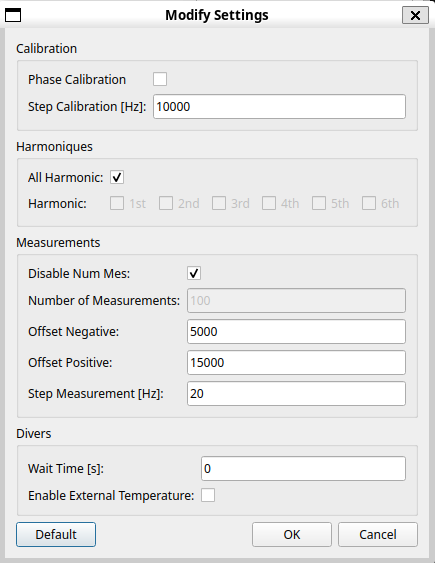
\includegraphics[width=\textwidth]{assets/figures/SettingsWater-Ethanol.png}
        \caption{Réglages pour l'eau, l'éthanol et le glycérol à 33\%.}
    \end{minipage}\hfill
    \begin{minipage}{0.48\textwidth}
        \centering
        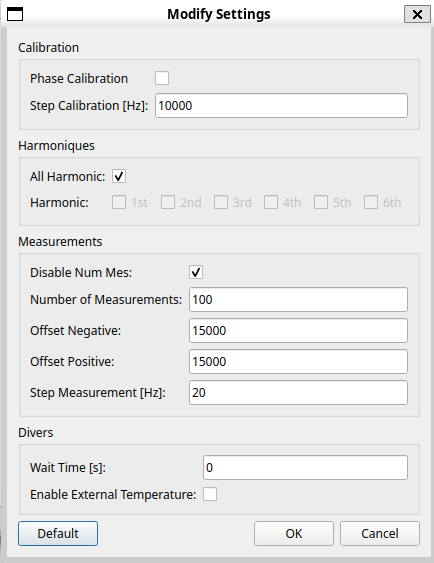
\includegraphics[width=\textwidth]{assets/figures/OilSettings.png}
        \caption{Réglages pour le glycérol à 55\%, le glycérol à 66\% et l'huile moteur.}
    \end{minipage}
\end{figure}

Le protocole suivant a été mis en place pour étudier l'influence de la température sur la réponse du capteur QCM :

\begin{enumerate}
    \item Remplir la cellule de mesure du QCM avec l'échantillon à tester.
    \item Régler la pompe péristaltique pour assurer une circulation constante du liquide autour du capteur.
    \item Démarrer l'acquisition des données (fréquence de résonance, amplitude, température).
    \item Augmenter progressivement la température du bain chauffant jusqu'à atteindre 45 °C, en veillant à ce que la vitesse de la pompe soit ajustée manuellement afin de garantir une montée en température régulière et contrôlée.
    \item Maintenir la température à 45 °C pendant quelques minutes pour assurer l'homogénéité thermique de l'échantillon.
    \item Refroidir ensuite le système en dessous de 20 °C, toujours en ajustant manuellement la vitesse de la pompe pour obtenir une descente en température constante.
    \item Enregistrer en continu les données du capteur QCM et de la sonde de température tout au long du cycle de chauffage et de refroidissement.
    \item Analyser les variations de la fréquence de résonance et de l'amplitude en fonction de la température.
\end{enumerate}

Le quartz utilisé pour cette mesure à une fréquance de base de 10Mhz est recouvert d'or voir le tableau \ref{tab:MatérielViscosité}.
Ce protocole permet d'observer l'effet de la température sur la réponse fréquentielle du capteur, tout en minimisant les gradients thermiques grâce à une circulation contrôlée du liquide.

\subsubsection{Protocole de mesure avec le viscosimètre}

Pour la mesure de la viscosité à l'aide du viscosimètre, la température de chaque échantillon est contrôlée par paliers successifs. À chaque étape, la température est stabilisée à une valeur cible avant de procéder à la mesure. Les températures choisies pour les paliers sont les suivantes :
\begin{itemize}[label=\textbullet]
    \item 20 °C
    \item 22 °C
    \item 24 °C
    \item 26 °C
    \item 28 °C
\end{itemize}

Pour chaque palier, une mesure de viscosité est réalisée une fois que la température de l'échantillon est stable. Ce protocole permet d'obtenir la courbe de viscosité en fonction de la température pour chaque liquide testé.

\subsection{Résultats}

Pour tous les résultats obtenus au moyen du capteur QCM, la troisième à harmonique (à 30Mhz) a été choisie car elle offre le meilleur signal. Les résultats de l'expérience se composent premièrement des mesures d'amplitude et de fréquence obtenues avec le capteur QCM, ainsi que de la température mesurée par la sonde PT100.  
Ils sont présentés dans la figure \ref{fig:Amplitude VS Température} pour l'amplitude et dans la figure \ref{fig:Frequence VS Température} pour la fréquence.

\begin{figure}[H]
    \centering
    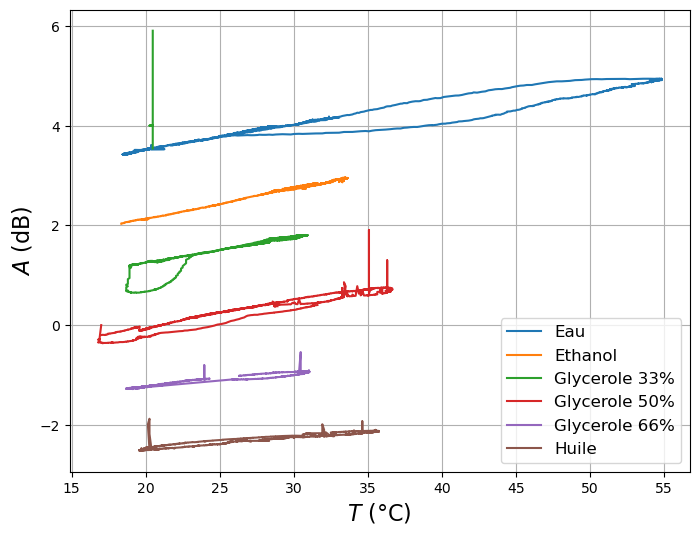
\includegraphics[width=\textwidth]{assets/figures/Amplitude-Temperature.png}
    \caption{Amplitude de la résonance en fonction de la température des différents échantillons}
    \label{fig:Amplitude VS Température}
\end{figure}

Il est intéressant de noter que, pour chaque échantillon, l'amplitude est essentiellement proportionnelle à la température, chaque échantillon présentant une pente qui lui est propre.  
La pente augmente lorsque l'amplitude de l'échantillon est plus petite.

On observe également une hystérésis pour chaque mesure. L'impact de celle-ci peut être réduit si la température varie plus lentement.  
Cette hystérésis n'est pas inattendue : le capteur de température PT100 ne mesure pas la température à la surface du quartz, mais celle du liquide dans la cellule de mesure, quelques millimètres au-dessus de la surface du quartz.

\begin{figure}[H]
    \centering
    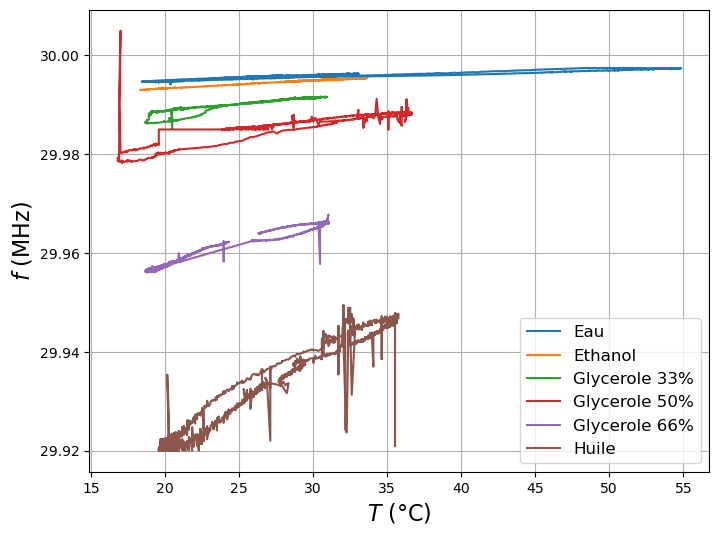
\includegraphics[width=\textwidth]{assets/figures/Frequ-Temperature.png}
    \caption{Fréquence de la résonance en fonction de la température des différents échantillons}
    \label{fig:Frequence VS Température}
\end{figure}

La figure \ref{fig:Frequence VS Température} présente la fréquence de résonance en fonction de la température des différents échantillons.  
Les observations sont similaires à celles faites pour l'amplitude : la fréquence de résonance augmente avec la température pour chaque échantillon, chaque échantillon ayant une pente propre.  
La pente de la fréquence est plus importante pour les échantillons dont la fréquence de résonance est plus faible.

Cependant, l'espacement entre les différentes courbes n'est pas le même, bien que l'ordre reste identique.  
Les échantillons ayant la fréquence la plus élevée, comme l'eau et l'éthanol, présentent un écartement plus faible sur les fréquences.

L’étape suivante consiste à mettre en relation la viscosité des échantillons avec l’amplitude et la fréquence de résonance.  
Pour chaque mesure de viscosité réalisée avec le viscosimètre, la température est enregistrée. Ensuite, pour chaque mesure, une amplitude ou une fréquence mesurée à la température la plus proche est associée.

\begin{figure}[H]
    \centering
    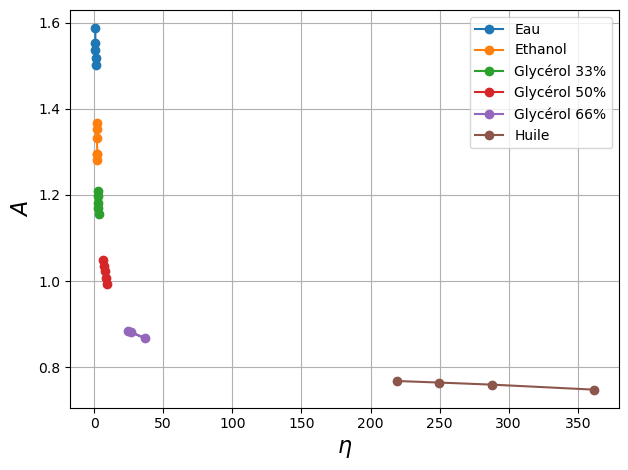
\includegraphics[width=\textwidth]{assets/figures/Amplitude-viscosite.png}
    \caption{Amplitude de la résonance en fonction de la viscosité des différents échantillons}
    \label{fig:Amplitude VS Viscosité}
\end{figure}

La figure \ref{fig:Amplitude VS Viscosité} présente l'amplitude de la résonance en fonction de la viscosité des différents échantillons.  
On constate que l'amplitude de la résonance diminue lorsque la viscosité des échantillons augmente.

On remarque aussi que, pour chaque échantillon, les amplitudes sont alignées avec celles des autres échantillons, ce qui suggère qu’un modèle unique pourrait décrire la relation entre viscosité et amplitude de résonance.

Les échantillons avec les viscosités les plus faibles, l'eau et l'éthanol, présentent une pente presque verticale, ce qui signifie que l'amplitude de résonance est très sensible à la viscosité.  
La pente de l'échantillon avec la viscosité la plus élevée, l'huile moteur, est proche de zéro.

\begin{figure}[H]
    \centering
    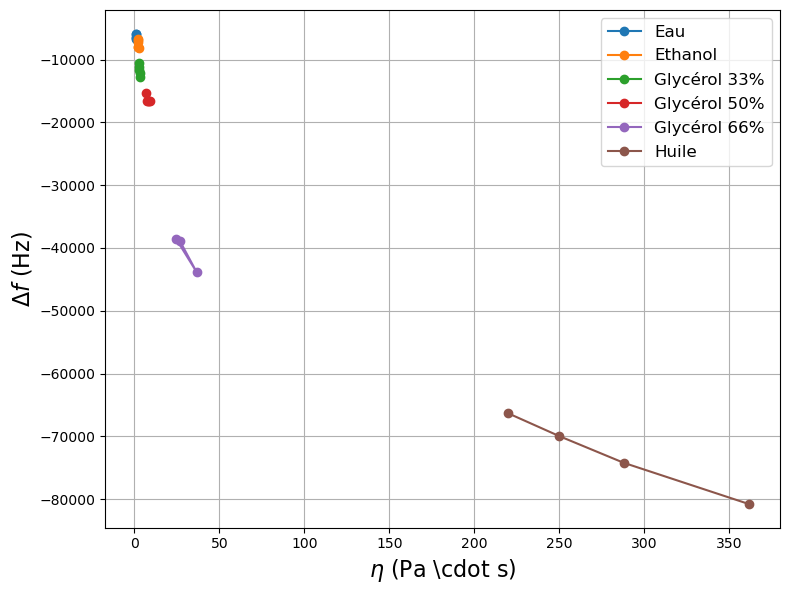
\includegraphics[width=\textwidth]{assets/figures/frequency-viscosity.png}
    \caption{Différence de fréquence en fonction de la viscosité des différents échantillons}
    \label{fig:Frequence VS Viscosité}
\end{figure}

Le graphique \ref{fig:Frequence VS Viscosité} présente la différence de fréquence en fonction de la viscosité des différents échantillons.  
Comme pour l'amplitude (figure \ref{fig:Amplitude VS Viscosité}), on constate que la différence de fréquence diminue avec l'augmentation de la viscosité.

Les pentes des fréquences suivent la même tendance que celles des amplitudes : les échantillons avec les viscosités les plus faibles ont des pentes plus importantes que ceux avec des viscosités plus élevées, bien que ces pentes soient moins marquées.

\subsection{Discussion des résultats}

Les résultats sont très intéressants dans la mesure où, une fois le modèle mathématique de la relation entre viscosité et signal de résonance déterminé, il sera possible de mesurer la viscosité d’un liquide par la simple mesure de l’amplitude de résonance du capteur QCM.  
C’est pourquoi nous avons cherché à déterminer la relation entre viscosité et fréquence de résonance.

Nous avons commencé par réutiliser l’équation \eqref{eq:frequence_resonance} qui relie la différence de fréquence à la viscosité.  
Cette équation suggère que la différence est proportionnelle à la racine carrée de la viscosité.  
C’est pourquoi les figures \ref{fig:Frequence carré VS Viscosité} et \ref{fig:Frequence carré VS Viscosité Zoom} représentent la différence de fréquence au carré en fonction du produit viscosité $\times$ densité des différents échantillons.  
L'espoir est que les données suivent une tendance linéaire. La pente devrait dépendre des caractéristiques du quartz.

\begin{figure}[H]
    \centering
    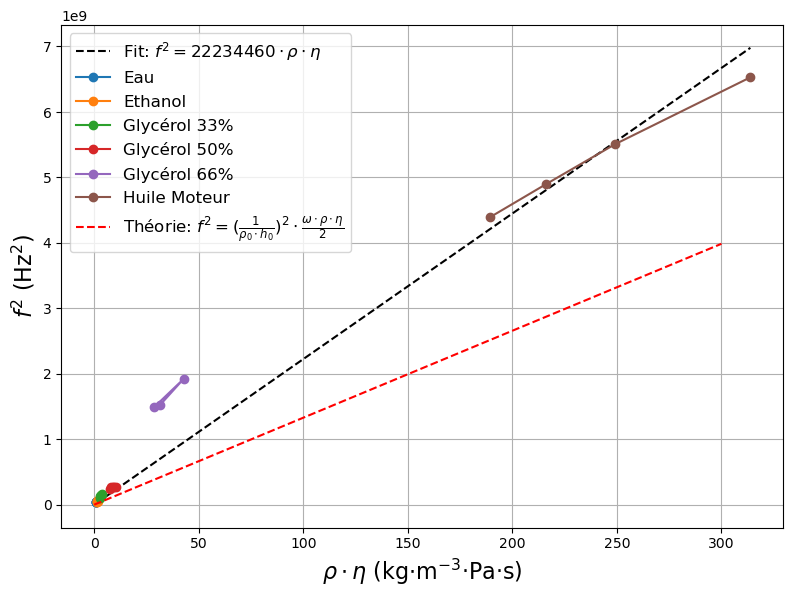
\includegraphics[width=\textwidth]{assets/figures/FrequVisc.png}
    \caption{Représentation de $\Delta f^2$ en fonction de la viscosité des différents échantillons}
    \label{fig:Frequence carré VS Viscosité}
\end{figure}

Sur la figure \ref{fig:Frequence carré VS Viscosité}, on pourrait penser que les données suivent une tendance linéaire, mais deux éléments remettent cette hypothèse en question.

Le premier est que l’échantillon de glycérol à 66\% de concentration s’écarte de la tendance générale.  
Il n’est pas clair si cela est dû à une erreur de mesure ou à un autre phénomène.

Le second est que les échantillons avec la viscosité la plus faible sont tellement rapprochés qu’il est difficile de distinguer les points à cette échelle.  
La figure \ref{fig:Frequence carré VS Viscosité Zoom} présente un zoom sur la partie gauche du graphique, où se situent les échantillons à viscosités faibles.

\begin{figure}[H]
    \centering
    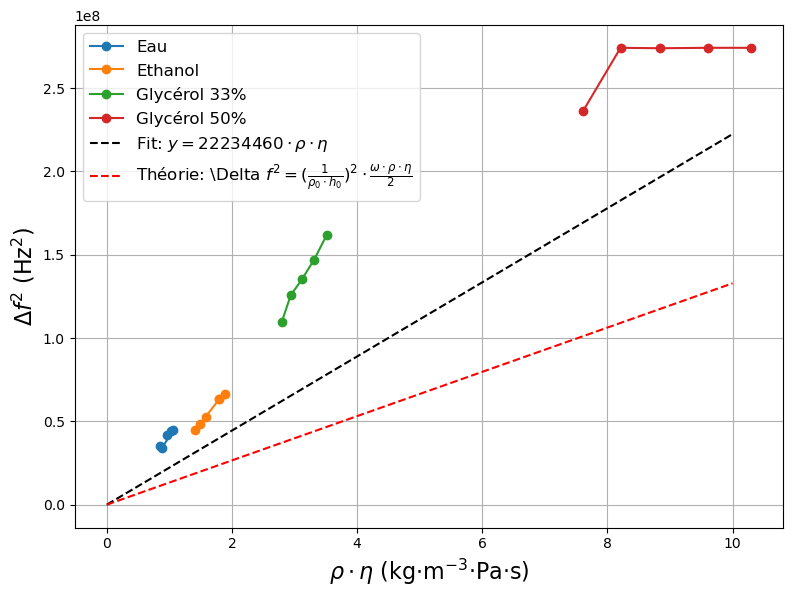
\includegraphics[width=\textwidth]{assets/figures/FrequViscZoom.png}
    \caption{Zoom sur la représentation de $\Delta f^2$ en fonction de la viscosité pour les échantillons à faible viscosité}
    \label{fig:Frequence carré VS Viscosité Zoom}
\end{figure}

Sur la figure \ref{fig:Frequence carré VS Viscosité Zoom}, les données semblent bien suivre une tendance linéaire, mais les écarts restent assez importants.  
Cela suggère que la relation entre la différence de fréquence au carré et la viscosité pourrait ne pas être strictement linéaire.  
Il faudra réaliser plus de mesures pour confirmer cette hypothèse, en utilisant par exemple d’autres proportions de glycérol et d’eau.

Les deux graphiques précédents affichent aussi la courbe que devrait donner le modèle théorique.  
L'écart est conséquent avec la régression calculée.  
Il est possible que cela soit dû aux caractéristiques du quartz, car pour calculer le modèle théorique, les caractéristiques fournies par le fabricant ont été utilisées.

\begin{figure}[H]
    \centering
    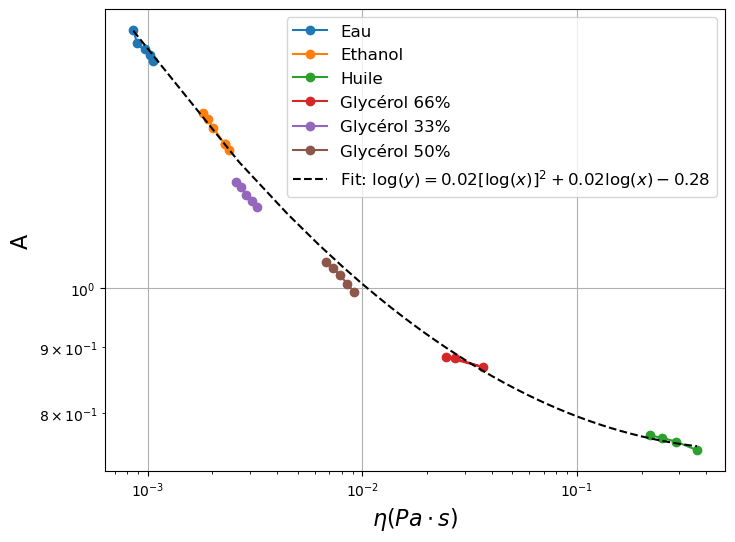
\includegraphics[width=\textwidth]{assets/figures/loglog.png}
    \caption{Représentation de $\Delta f^2$ en fonction de la viscosité des différents échantillons sur une échelle logarithmique}
    \label{fig:loglog}
\end{figure}

La figure \ref{fig:loglog} présente l’amplitude de la réponse en fréquence en fonction de la viscosité des différents échantillons, sur une échelle logarithmique.  
Un ajustement a été réalisé, de la forme suivante :
\begin{equation}
    \Delta \log(f) = a \cdot \log(\eta)^2 + b \cdot \log(\eta) + c
\end{equation}

Cette forme ne correspond à aucune des équations connues décrivant la relation entre viscosité et fréquence de résonance.  
Cependant, elle permet tout de même de prédire l’amplitude d’une mesure.

\section{Gélification}

Les mesures de gélification sont utiles car elles permettent d'observer les transitions de phase d’un état liquide vers un état gélatineux. La gélatine bovine est utilisée car ses changements de phase se produisent à des températures proches de la température ambiante, ce qui correspond bien à la plage de fonctionnement du capteur QCM.

\subsection{Matériel}

\begin{table}[H]
    \centering
    \begin{tabular}{|l|l|l|}
        \hline
        \textbf{Matériel}         & \textbf{Fabricant}   & \textbf{Numéro de série} \\
        \hline
        Open QCM - Q1             & Open QCM              &   \\
        Module électrochimique    & Open QCM              &   \\
        Quartz 5 MHz             & Open QCM              &   AT5-14-12-SS316-WRAP\\
        Bain chauffant            & Stuart                &  R00199487 \\
        Pompe péristaltique       & LaerdFluid            &  BQ8oS \\
        Sonde PT100               &                       &   \\
        \hline
    \end{tabular}
    \caption{Liste du matériel utilisé pour la mesure de gélification}
    \label{tab:materielGelification}
\end{table}

\begin{table}[H]
    \centering
    \begin{tabular}{|l|l|l|}
        \hline
        \textbf{Produit} & \textbf{Fabricant}   & \textbf{Numéro de série} \\
        \hline
        Eau distillée    & HEIG-VD              &   -           \\
        Gélatine bovine  & Sigma-Aldrich        &   G9382-100G  \\
        \hline
    \end{tabular}
    \caption{Liste des produits utilisés pour la mesure de gélification}
\end{table}

\subsection{Protocole}


La préparation de la solution consiste à dissoudre la gélatine dans de l’eau chaude. Un rapport de 7,5 g de gélatine pour 100 g d’eau a été utilisé. L’eau est chauffée à 60 °C, puis le mélange est agité pendant 30 minutes afin d’assurer une dissolution complète.

Le protocole mis en œuvre pour étudier la gélification est le suivant :
\begin{enumerate}
    \item Préparer la solution de gélatine comme décrit ci-dessus.
    \item Remplir la cellule QCM avec 10ml de la solution chaude.
    \item Démarrer l’acquisition des données à l’aide du capteur QCM.
    \item Refroidir progressivement la solution à l’aide du système de refroidissement décrit précédemment.
    \item Observer les variations de la fréquence de résonance tout au long du processus de gélification.
\end{enumerate}
Le montage est le même que celui expliqué dans le chapitre \ref{chap:Gestion de la température}.

Le quartz utilisé pour cette mesure à une fréquance de base de 5Mhz est recouvert d'acier inoxydable, voir le tableau \ref{tab:MatérielViscosité}.

Les paramètres utilisés pour les mesures sont présentés sur la figure~\ref{fig:SettingsGelification}. Ces réglages correspondent à ceux utilisés pour l'acquisition des données lors de l'étude de la gélification.

\begin{figure}[H]
    \centering
    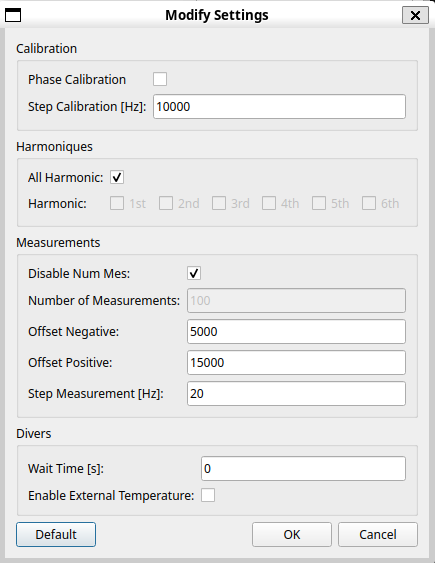
\includegraphics[width=0.6\textwidth]{assets/figures/SettingsWater-Ethanol.png}
    \caption{Paramètres de mesure utilisés pour la gélification}
    \label{fig:SettingsGelification}
\end{figure}

\subsection{Résultats}

Les résultats de la mesure de la gélification sont présentés dans la figure \ref{fig:Frequence gelification}. Ils se trouvent à la troisième harmonique du cristal (15 MHz) car c'est la que se trouve le signal le plus propre. 

Lorsque le liquide est refroidi, un changement de la pente entre la fréquence de résonance et la température est visible aux alentours de 25 °C. 

Au-dessus de cette température, la pente est similaire à celle de l'eau, en dessous la pente est plus importante.  

Ce changement indiquerait un changement d'état du gel, passant de l'état liquide à l'état gélifié.

Une fois que le liquide a atteint sa température minimale et que de l'eau chaude circule autour du capteur, la température augmente plus vite que la fréquence de résonance. Un autre point de changement de phase est visible aux alentours de 32 °C, ce qui correspondrait à la température de liquéfaction de la gélatine en liquide.

\begin{figure}[H]
    \centering
    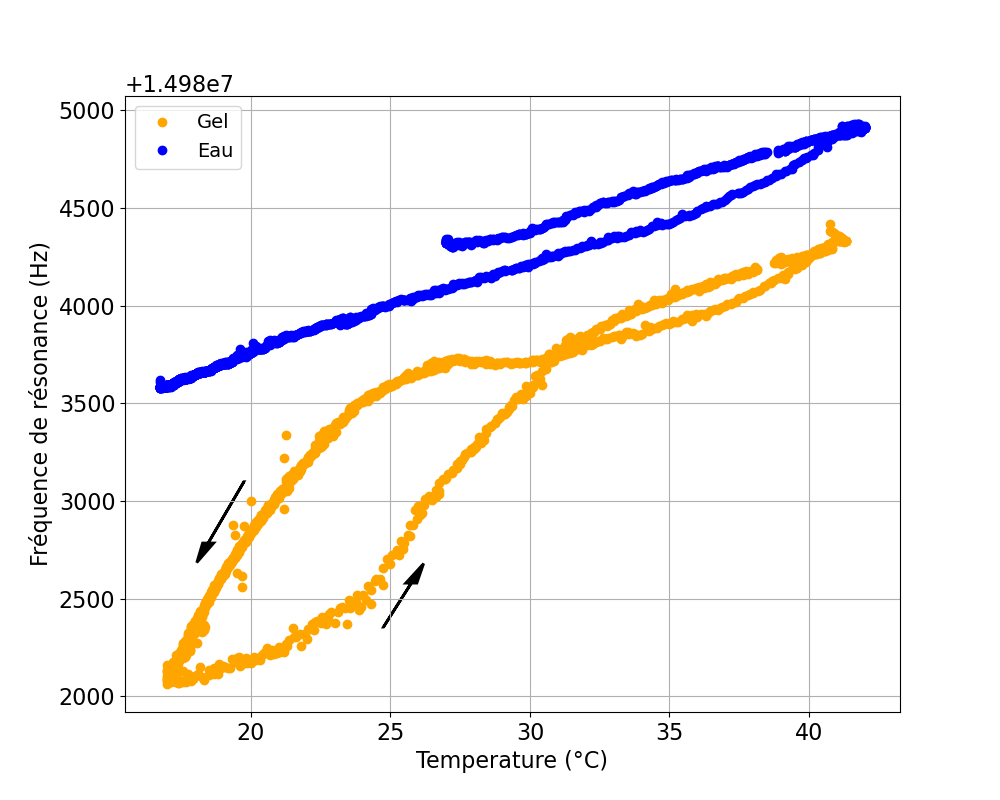
\includegraphics[width=0.8\textwidth]{assets/figures/gel.png}
    \caption{Fréquence de résonance en fonction de la température pour la mesure de la gélification}
    \label{fig:Frequence gelification}
\end{figure}

\subsection{Discussion des résultats}

En comparant avec les données de la littérature \cite{SHA2019163}, la température de gélification varie entre 5 °C et 20 °C, tandis que la température de fusion se situe entre 20 °C et 30 °C. Ces données ont été mesurées avec de la gélatine porcine. En effet, la température d’extraction, parmi d’autres variables, a un impact sur la température de solidification.

Les températures mesurées avec la microbalance à quartz présentent un léger écart par rapport aux données de la littérature. Cela pourrait s’expliquer par la position du capteur de température : en effet, ce dernier est situé sur un PCB, en dessous du quartz, ce qui entraîne un décalage avec la température réelle à l’intérieur du récipient. Cette différence pourrait donc justifier l’écart observé.


